\documentclass{llncs}
%\documentclass{article}
\usepackage[utf8]{inputenc}
\usepackage{cite}
\usepackage{verbatim}
\usepackage{graphicx}
\usepackage{wrapfig}
\usepackage{listings}

\title{Performance of two different ontological and data access methods}
\author{Magn\'{u}s D\ae hlen \and Kjetil Kjernsmo}
\institute{Department of Informatics,
Postboks 1080 Blindern,
N-0316 Oslo, Norway \email{\{magnudae,kjekje\}@ifi.uio.no} }


\subtitle{---Draft submitted to COLD 2014---}


\begin{document}
\maketitle

\begin{abstract}
  We evaluate two different approaches that have been used in the
  literature and in practice by different groups publishing metadata
  about cars when consumed by a prototype application. These
  approaches are characterized by a generic vs. domain specific
  ontology; by a constrained tree-oriented API vs. openly queryable
  data; encouraging vs discouraging reasoning, etc.  We have
  implemented a prototype application where a potential user may query
  selected properties of cars, and we investigate how the different
  choices made by the original designers influence the performance of
  the application. For the evaluation, we employ the statistical
  disipline of Design of Experiments.

\end{abstract}

\section{Introduction}

The retrieval of information from different sources and then combine
them to allow a user to find a certain combination of properties that
suit their purpose is an archetypical Semantic Web use case. We have
chosen to focus on a product selection use case, specifically on cars,
since some car manufacturers have embraced the Semantic Web vision and chosen
to share detailed data on their products.

The findings, we assert, have a broader validity, given the generic
nature of the problem they are trying to solve, and so our
recommendations should have broad relevance to similar use cases.

We present two different approaches. One is promoted by Renault, see
\cite{SemWebAppRes} and \cite{ren1}. They have developed the
Configuration Ontology (CO) \cite{confOnt}, and developed an API to allow
users to traverse the RDF graph to find a smaller result set of cars.
The ontology focuses on building an RDF graph to represent all valid
configurations for a product model with component constraints.  It is
also made so that it is not needed to do any reasoning to get a valid
result set.  They call it a traversal of \emph{Configurations} which
will end up with a \emph{Partially Defined Products}
(PDP)\footnote{Partially Defined Product is a way of defining a
  product without using all of the features. For instance a car which
  may have many features, but we describe it as a car with mp3 and
  sunroof.}.  Their method insists there is a starting point, which is
a car model. From there, there is a \emph{lexicon} which can be used
to choose different specifications which may lead to a valid
configuration. There are also stated if some specifications are
impossible in the current configuration.  These are represented by
either the \textsf{co:possible} or \textsf{co:impossible}
property. Furthermore, string comparison must be used to check if a
certain specification is representing for instance fuel type.


The other approach was made by Martin~Hepp in collaboration with
Volkswagen resulting in the Car Options Ontology (COO) \cite{COO} and
the Vehicle Sales Ontology (VSO). They are designed to be used in
combination with GoodRelations, also designed by Hepp. When using COO,
one defines a base car model, and a \emph{trim} is defined on the
base, while a derivative car model should specify compatibilities and
constraints between configurations, e.g. an electrical car does not
have a conventional gear box.

A central difference with these ontologies is that CO allows the
configuration to be defined in terms of classes, whereas VSO
represents them with properties, for example:
\begin{lstlisting}[basicstyle=\tiny, frame=single]
#CO representation of fuel type
:var_PT1628  a           co:ConfigurationVariable , owl:Class ;
        rdfs:label       "Fuel Type"@en ;
        co:confVarId   "PT1628" ;
        co:hasValue    
	    <http://uk.co.rplug.renault.com/product/gen/spec/PT1628_diesel/-#this> .

#VSO representation of fuel type
daim:A200CDI vso:fuelType daim:A200CDI_fuelType_Diesel_fuel .
\end{lstlisting}



We shall compare them to find their strengths and
weaknesses. Each approach contains an ontology and has its own way of
representing data.  To make this comparison we have used data about
the same domain, data about car models and their component
constraints.  The first approach is a generic ontology. By generic it
means that it can be used to represent any product model with
component constraints. The second approach is a domain specific
ontology which as the name implies, is only applicable with one
particular domain. In this thesis that domain is about car models.

We will also show how to create a viable web application which
utilizes such complex data, mainly for the purpose of conducting
performance tests to determine the weaknesses of each approach. This
will be done with complex data found on the web today from different
car manufacturers.  With performance we mean the response time between
a HTTP post operation against the application and when
the application presents the user with an answer. The application will
contain the possibility to do HTTP posts against both approaches.

There will be several options on how to query the data because of all
the different specifications.  That is why we have chosen to use the
testing approach \emph{Design of Experiments} (DoE). This approach
will be further explained alongside the results in
Section~\ref{Results}. The evaluation will be based on four
experiments testing several aspects of the approaches. They will help
us determine what kind of factors are significant to the performance.

\section{Related work}
Complex products and specifying configurations has been a research
topic for over a decade.  The possibility to personalize more and more
products is why several research articles have proposed different
approaches on how to handle these configurations. Most of the research
are around finding the ultimate solution with a specification
system. In 1999, M. Aldanondo et. al proposed how to structure a
system to handle configurations and their constraints. This included
proposed definitions for products, configurations and
configurators. The paper focused on making a generic solution to fit
several manufacturers.~\cite{OldConf} In a newer article,
H. Afsarmanesh and M. Shafahi (2013) proposed a complex product
specification system.~\cite{NewConf} This include object modelling and
a user interface. They have focused on supporting stakeholders in the
specification process.

Unfortunately these articles do not present any research done with
semantic technologies. The use of semantic technologies on complex
products is a young field of research. The only thing done here is
what Renault and Volkswagen have presented. Both of these car
manufacturers have presented the public with two different
solutions. They have also shown how to present the data on the web and
the complexity around their solutions.

The Volkswagen solution builds upon GoodRelations, which is a web
vocabulary for e-commerce and was launched in 2008 and is now
widespread. GoodRelations.~\cite{GR} GoodRelations can be used for
detailed information about products to be sold online.

% TODO: Har litt på følelsen at dette blir for tynt for et paper,
% mulig det burde vært mer generelt om Goodrelations, etc. Vi kan jo
% bare se det an.

\section{Evaluation platform}

We set out to evaluate different approaches based on a real use case
where a user is seeking to buy a new car based on detailed data
published by car manufacturers. Note that the implementation is not
itself an important contribution, it is the evaluation that is the key
contribution. Today only Renault, of all the car manufacturers, has
opened their data using semantic technologies. Volkswagen had their
data published until the start of 2013, but unfortunately they
canceled their Semantic Web project and the data were removed.
Fortunately, their ontologies are still open for the community to
use. Eventually, we found Daimler very forthcoming, as they offered
data about their A- and B-class cars.  The Daimler data used a custom
XML-based format, so we lifted the data using a \textit{python} script into the
ontologies developed by Martin Hepp and Volkswagen.

To be able to put large stress on the application, which again would
allow us to bring out key strengths and weaknesses of the two
different approaches, we chose to create an application where a user
choose several or all car options specifications.

The application was implemented using Apache Maven, Spring and Apache
Tomcat as well as Jena.

To align the above ontologies, we used SPARQL CONSTRUCT statements
from the lexicon to each specification.

The application present users with a web interface where they can
input values for any specification they might want to search
for. There the user can input values for the different specifications,
for instance fuel type or CO$_2$ emission. After a user is done
choosing specifications he can execute the actual car model
search. The application extracts the data from the form and comprises
it into another format that can easily be used later on. The next step
begins in the search module. Here it starts a thread for each possible
car model to execute each individual search. In the end the user is
presented with a set of valid models to choose from, which contain the
chosen specifications, e.g. the user have searched for a model with
diesel fuel, automatic transmission, four or more gears and a maximum
of six seats.

Some pre-computations are done to make the application a little
more effective. This includes extracting all the model names from both
ontologies, initiate all possible partially defined products as a
PartialCar object and creating some internal structure. These
pre-computations were done so that it would be possible to present the
user with the name of each car model, not just the URI. We will also
describe more in depth how the car model search is done later on.


\section{Experiments}\label{Results}

To perform a statistically sound experiment, we turn to techniques
from statistics known as Design of Experiments (DoE). For an
introduction to the use of DoE in Semantic Web research, see~\cite{Kjern}.

\subsection{Planning the experiment}
Like other approaches, there are several steps in doing experiments with
DoE.  First one has to state an objective which is important to give
the experiment a purpose.  The next step is to choose a response. The
response is the experimental outcome or observation. There may be
multiple responses in an experiment. In this experiment there will be
one response and that is the response time on a HTTP post against the
application.  These first two steps are the same for all the
experiments in this thesis.

The next two steps of planning an experiment is specific to each
experiment itself. This means that these steps will be described more
in depth in each experiment because it may vary depending on the
actual experiment.  The third step in planning an experiment is
choosing factors and levels. This is a key part of DoE. A factor is a
variable that is studied in the experiment, and to be able to study
this factor it is needed to use two or more values of this
factor. These values are referred to as levels.  The levels will allow
us to examine the influence of each factor. It is important to
identify the key factors in the planning stage. This is to get the
maximum effect out of the experiment.  Factors may be
\emph{quantitative} or \emph{qualitative}. Quantitative factors
are often numerical values that represent an interval. For instance
the weight of a car is considered a Quantitative value. Qualitative
factors are predefined values within a known set of values.  In our
case a Qualitative factor can be the type of fuel, for instance
Diesel.

The fourth step in planning is to choose the experimental plan. Here
we will use one specific approach. The approach is called \emph{full
  factorial experiment} which we will go into more detail about in the
next sub-section. There are other approaches like fractional factorial
experiment, but they were not applicable or relevant to this thesis.
The last three steps of planning the experiment are performing the
experiment, analyzing the output and in the end drawing
conclusions. More about these steps will be taken individually at each
experiment.~\cite{PlanExp}


\subsection{Full factorial experiment}
A full factorial experiment is when one got $k$ factors and $n$ amount
of levels. This means that there is $n^k$ \emph{factorial designs}
which result in $n^k$ designs to execute.  We have chosen only
two-level experiments for this research, but the factors may vary. This
means that we will use a $2^k$ full factorial design for every
experiment. The experiments consist of $2^k$ combinations with $k$
factors. For instance if we have three factors where every factor got
two levels we get $2^3$ designs, also called \emph{runs}. This results
in a \emph{planning matrix} that shows the actual runs in the
experiment.




\subsection{Running the experiments}
In this section we will present several experiments with different
amount of factors.  The objective is to find out how the ontologies
will perform in comparison and identifying which factors affect the
outcome of each experiment. We did the ontology alignment and
development of the application to prevent the loss of precision with
either ontology.

In the experiments the definition for VSO/COO is \textsf{-vso} and for
CO is \textsf{-co}.  These two definitions stand for which ontology
are tested in a particular run. In practice this means that when we
send in the keyword \textsf{-vso} we only run the specification search
against the car models represented by VSO/COO, in our case the data
from Daimler. This is referred to as the ontology factor in each
experiment and is a factor in all the experiments which are presented
in this thesis. The ontology factor represents the difference in how
the data are represented and how the ontologies are structures, and
with this factor we want to determine how this affects the overall
performance.  We have programmed the application so that the querying
of the ontologies are done as similar as possible on both levels. This
was done to eliminate any interference from the application.

First, we created the planning matrix and then executed each run as a
HTTP post. To do this we needed to make a small script to calculate
the $2^k$ runs and perform the HTTP posts. We used the programming
language \emph{Python} with the
DoE\footnote{http://pythonhosted.org/pyDOE/} package.

The \emph{payload} is a dictionary of all the values to post to the
application.  After the request we saved the response which contained
the response time of a run. After each request we saved the run plus
the response time and wrote it to file on CSV format. To evaluate the
result we used the programming language R with the packages
\textsf{DoE.base}~\cite{DoEBase}, \textsf{FrF2}~\cite{FrF2} and
\textsf{BsMD}~\cite{BsMD}. R allowed us to parse the CSV files created
from the experiments and output them in two types of graphs.  A
similarity with all the experiments were that they all contained at
least the factors ontology, transmission and fuel type.

To evaluate the graphs we have used a method in the \textsf{FrF2} R
package called \textsf{DanielPlot}. This method assumes that the
estimated effects are normally distributed with means equal to the
effects. The means of all estimated effects are zero. Resulting in a
plot where the estimated effect would end up on a straight line. This
plot is then testing whether all the estimated effects have the same
distribution. All deviations of the straight line indicates a
significant factor. In our results we have used the absolute value of
the effects, also called a half-normal plot. The advantages of using
the half-normal plot is that all large estimated effects will end up
in the top right corner. This means that the highest performance
significance will end up in
the top right corner.~\cite{Plotting} \\
Here is a quick explanation of the axes shown in each graph.  The X
axis will show the absolute effect of each factor, shown in time. The
values on the X axis is represented in seconds which means that the a
plot will have a significance measured in seconds.  The Y axis shows
the half-normal scores. There are two way of representing the graph
and that is with either half-normal plots or normal plots. With
half-normal the effects on the X axis are shown with the absolute
effect. This means that all factors are placed with a positive
half-normal score. This is to avoid visual misleading scores because
with the normal scores, deviations from the line on negative scores
might confuse the reader who are evaluating the charts.  The scores
them selves are a measure for which factor that is the most
significant.  We have also set  the significance level at $\alpha =
0.05$, where \textsf{DanielPlot} is using Lenth's method for the
analysis of unreplicated factorials. % TODO: Need a citation here.

For brevity, we will use abbreviations given in Figure~\ref{facandabbrev}.

\begin{wraptable}{l}{0.35\textwidth}
    \begin{tabular}{ | l | l |}
    \hline
    {\bf Factor} & {\bf Abbrev} \\ \hline
   Ontology & \textsf{O} \\
   Fuel Type & \textsf{FT} \\
   Transmission & \textsf{T} \\
   Weight & \textsf{W} \\
   Total Weight & \textsf{WT} \\
   Emission & \textsf{E} \\
   Nr. of Gears & \textsf{G} \\
   Seating Capacity & \textsf{SC} \\
   Fuel Consumption & \textsf{FC} \\
   Doors & \textsf{D} \\
\hline
    \end{tabular}
\caption{Factors and their abbreviation}\label{facandabbrev}
\end{wraptable}


We ran several experiments, both randomized and unrandomized
experiments, with 3, 4, 6 and 10 factors. Here, we report on the
unrandomized 3 and 10 full factorial experiments:
  
\subsubsection{Experiment with three factors}
We first made a very simple three factor experiment. The main goal here was
to see how the ontologies behave with a small amount of querying and
factors. We chose to start with a small experiment using only
simple factors which had few possible values. That is why we chose
transmission and fuel type as factors as well as the ontology
factor. With these three factors we got $2^3$ number of runs. This
experiment was also replicated four times to get the most accurate
results.  The results were calculated by finding the average response
time for each run between all four replications.

The next step was to create the planning matrix for this
experiment. Table~\ref{3factor} shows all the 8 runs for the
experiment with three factors.  After each run the response time were
logged to that particular run. The response time were then used to
check for significant effect when the experiment were evaluated
\begin{wraptable}{l}{0.67\textwidth}
    \begin{tabular}{ | l | l l l |}
    \hline
    {\bf Run} & {\bf Ontology} & {\bf Fuel type} & {\bf Transmission} \\ \hline
	1 & -vso & Diesel & Automatic Gearbox \\ \hline 
	2 & -co & Diesel & Automatic Gearbox \\ \hline 
	3 & -vso & Unleaded Petrol & Automatic Gearbox \\ \hline 
	4 & -co & Unleaded Petrol & Automatic Gearbox \\ \hline 
	5 & -vso & Diesel & Manual Gearbox \\ \hline 
	6 & -co & Diesel & Manual Gearbox \\ \hline 
	7 & -vso & Unleaded Petrol & Manual Gearbox \\ \hline 
	8 & -co & Unleaded Petrol & Manual Gearbox \\ \hline 
    \end{tabular}
    \caption{Planning matrix for experiment with three factors and
      their levels.}\label{3factor}
\end{wraptable}


Like the rest of the experiments we used DanielPlot to evaluate and a
package in R to visualize the result. Figure~\ref{3factorGraph}
shows only one significant factor, namely the \textsf{O} factor in the
upper right corner. In Table~\ref{3factorEffect}
we can see the time effects from largest to smallest.  We see that the
ontology factor has the largest effect on approximately 2.2 seconds
which means that one of the ontologies overall is 2.2 seconds
faster. By reading the results from the linear model it is the factor
level \textsf{-vso} which has an overall faster response time.

\begin{wraptable}{l}{0.25\textwidth}
%\vspace{-25pt}
    \begin{tabular}{ | l l |}
    \hline
    {\bf Factors} & {\bf Effect}  \\ \hline
	  O     & 2.246\\ \hline
	  O:T    &0.454 \\ \hline
	  O:FT:T &0.453 \\ \hline
	  T      &0.451 \\ \hline
	  FT:T   &0.450 \\ \hline
	  O:FT   &0.124 \\ \hline
	  FT     &0.118 \\ \hline
    \end{tabular}
\caption{Table of absolute effects for the three factor experiment}\label{3factorEffect}
%\vspace{-25pt}
\end{wraptable} 


\begin{wrapfigure}{l}{0.65\textwidth}
 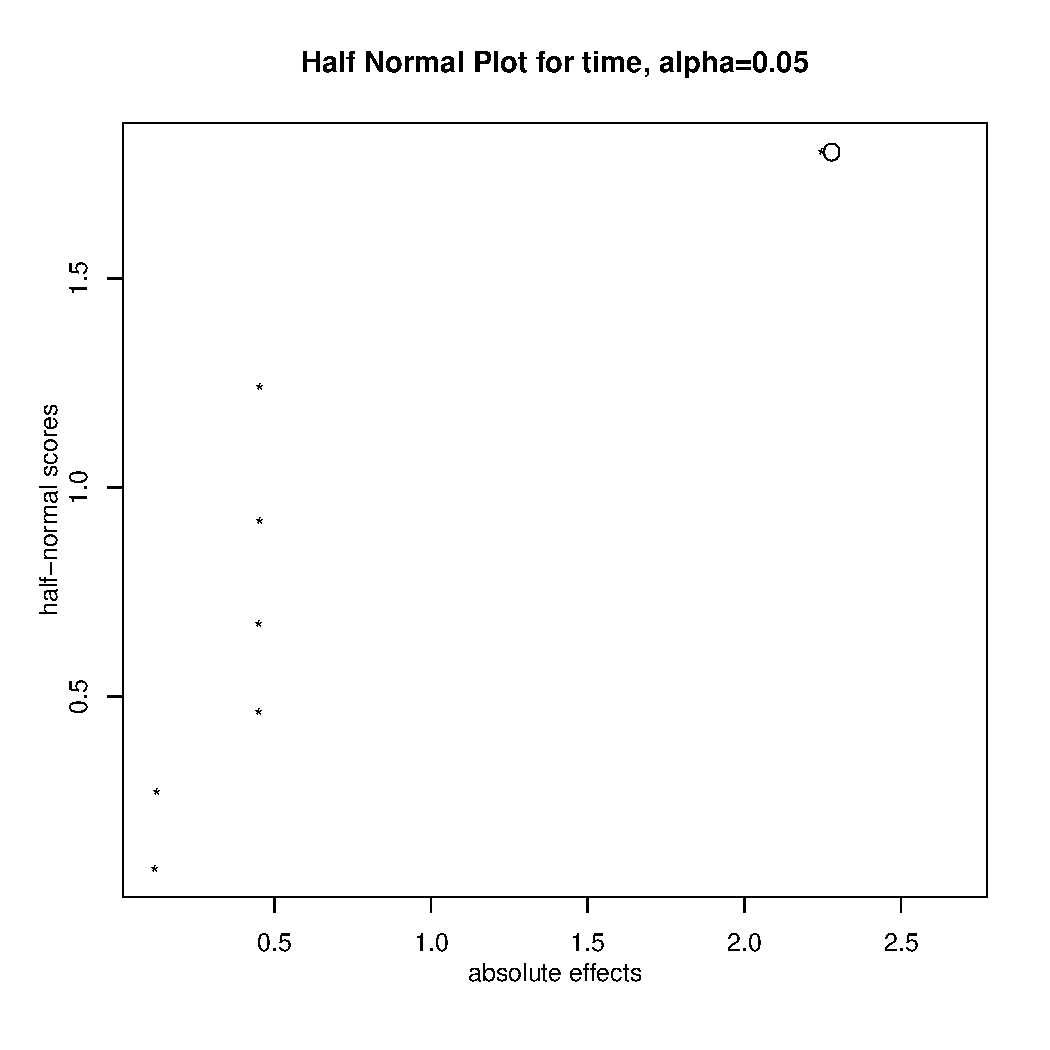
\includegraphics[width=8.5cm, height=7cm]{2factorfinal.pdf}
  \caption{Resulting graph for the three factor experiment}\label{3factorGraph}
\end{wrapfigure}


\subsubsection{Experiment with ten factors}
The last experiment we did was a ten factor experiment. The goal here
was to see which factors would be deemed significant in a complete car
model search. With the results from this experiment we could discuss
several aspects of using the different ontologies.  Here we added 4
new factors in comparison to the six factor experiment. The newly
added factors were \emph{weight}, \emph{nr. of doors},
\emph{nr. of seats} and \emph{fuel consumption}. We used the same
approach here as in the previous experiments to calculate the average
value for the new factors. % TODO: Explain more how the levels were set?
With 10 factors the amount of
runs were $2^{10}$, which made the planning matrix too big to show here.

In the graph~\ref{10factorGraph} we can see the results from running
all the 1024 runs.  We can see that there are a lot of significant
effects present here. There are more than any of the previous
experiments, but it is also more factors and factor interactions.
Unfortunately there are so many significant factors that there are
some of them that are illegible, but most of them have a low impact on
the significance graph.  In Table~\ref{10factorEffect} we can see the top
twenty absolute effects. We can see that emission also here are present in a lot of the
entries, but so is ontology as well. The new thing here is the fuel
consumption has entered the most significant factors, and is by itself
higher than emission. The linear model again tells us that the option
\textsf{-vso} has a significantly lower response time than
\textsf{-co}

When we accumulated the results from all the runs we ended up with the
total amount of response time to be approximately 30095 seconds, which
is 8 hours, 21 minutes and 35 seconds.  This were the total response
time after running all the runs. This did not take into account all
the other steps during the experiments which took time, like writing
results to file and initiating the application.  This discouraged the
replication of the experiment due to the size and was also a reason
why we did not do experiments with more factors.




\begin{wraptable}{l}{0.25\textwidth}
\vspace{-25pt}
    \begin{tabular}{ | l l |}
    \hline
    {\bf Factors} & {\bf Effect}  \\ \hline
      O & 58.17 \\ \hline
      E:FC & 45.69 \\ \hline
      O:E:FC & 45.55\\ \hline
      FC & 38.61\\ \hline
      O:FC & 38.56\\ \hline
      O:E & 35.40\\ \hline
      E & 35.38\\ \hline
      O:T & 33.12\\ \hline
      T & 33.12\\ \hline
      O:T:E:FC & 29.31\\ \hline
      T:E:FC & 29.30\\ \hline
      O:T:FC & 28.24\\ \hline
      T:FC & 28.23\\ \hline
      O:T:E & 25.31\\ \hline
      T:E & 25.30\\ \hline
      WT:E & 11.92\\ \hline
      O:WT:E & 11.89\\ \hline
      O:WT:FC & 11.72\\ \hline
      WT:FC & 11.71\\ \hline
      O:D:E & 10.12\\ \hline
    \end{tabular}
\caption{The top twenty significant absolute effects of the ten factor graph}\label{10factorEffect}
      \vspace{-25pt}
\end{wraptable}


\begin{figure}
 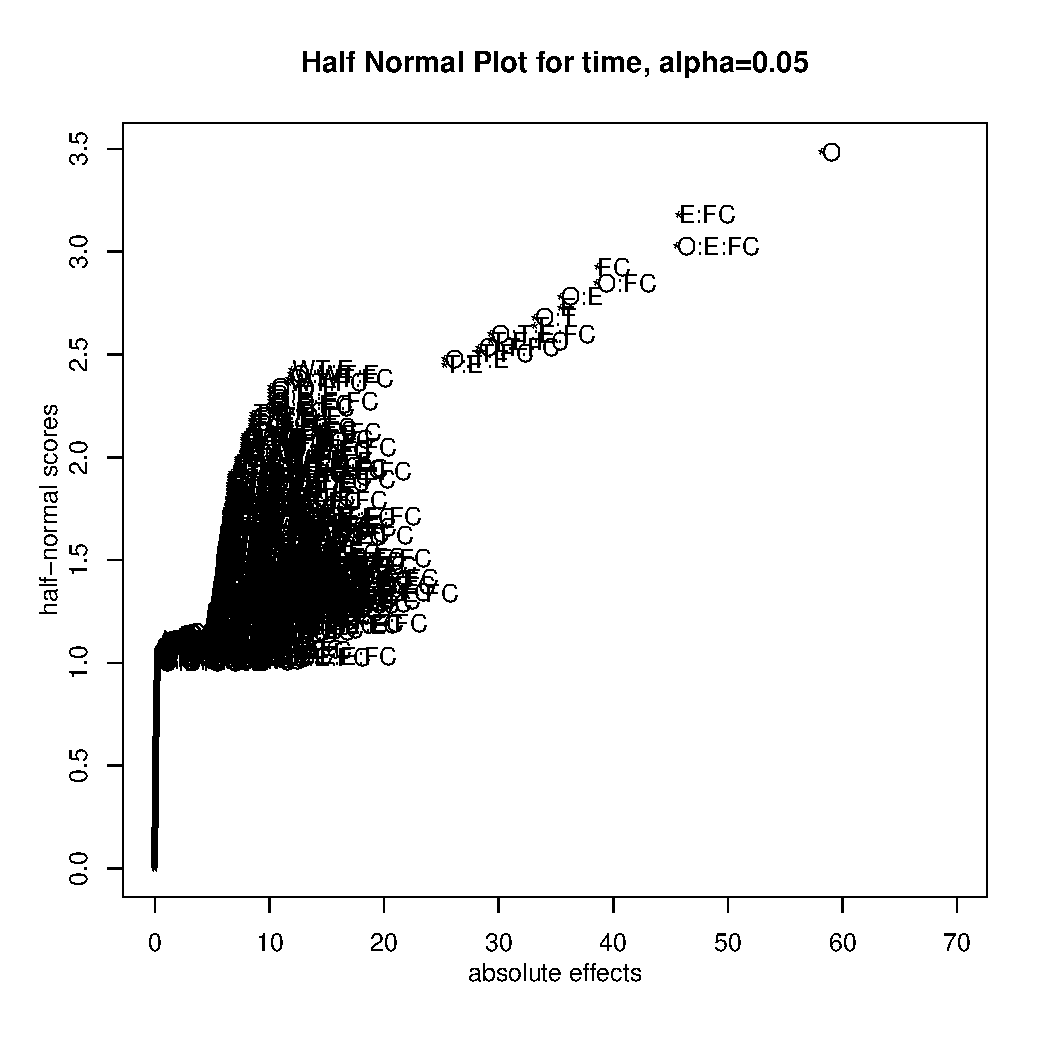
\includegraphics[width=14cm]{10factorAvarageDanielPlot.pdf}
  \caption{Resulting graph for the ten factor experiment}\label{10factorGraph}
\end{figure}

\section{Discussion}

We will discuss the results in terms of \emph{representation} and
\emph{structure}. The structure is the ontology definitions from
classes to properties.  The representation is how the actual data is
represented with each ontology. For instance, how the fuel type
\emph{Diesel} is represented.

\subsection{The small scale experiments}
The first experiment, using only three factors, was done to simulate a
small workload on the ontologies. This can represent an application
that present the user for a specification one at the time. The
configurator Renault has on their web page does exactly
that.\footnote{\url{http://www.semanlink.net/2012/cold/configurator.html}}
Our application made the workload on both ontologies to be as equal as
possible.  The only difference from a programming perspective was that
with CO we had to move to a new configuration URI after each
specification choice.

In the Figure~\ref{3factorGraph} we can see that only one significant
effects, the O factor. We saw in Table~\ref{3factorEffect} that the
Configuration Ontology was almost two seconds slower than the VSO/COO
runs.  Three out of four CO runs kept the response time around two
seconds, but one run had to use approximately 3.5 seconds which
resulted in an average run time of $\approx2.3$ seconds.  In a study
done to research the amount of time a user would be willing to wait,
they found out that the tolerable waiting time for any information
retrieval was approximately 2 seconds.~\cite{waitTime} This means that
with three factors we were still within the time frame for a good user
experience.

One reason that CO was slower than VSO/COO for this experiment is that
all the car models represented with CO is placed in a separate RDF
graph. Each model had their own lexicon with all the information.
This means that an application has to retrieve in all 22 RDF graphs,
the amount of cars Renault has present in their API. These 22
retrievals are done right after a HTTP post is detected. This differs
from how the cars in VSO/COO are represented. There it is one RDF
graph per base model, which means that there were only two RDF graphs
to retrieve.  In our application this results in 20 more RDF graph
retrievals with CO than VSO/COO and because the three factor
experiment was so small, it had a higher impact than in the later
experiments.

Another factor that would influence the results is the amount of
values the search has to iterate over.  We have found that CO have
$0.54$ more fuel types on average to iterate over and $0.3$ more
transmissions. This is not a lot, but can account for some delay in
the response time.

\subsection{The large scale experiments}
The last experiment we define as a large scale experiment. This is
because the workload and time consumption were significantly larger
than the previous experiment. This experiment were done
to simulate a workload for an application were one could define all
the specifications at once. Defining all specifications means that a
user can query for all specifications that may be present in a product
model.

This experiment had seven more factors than the three factor experiment.  We chose to add
factors which represented specifications that were present in every
car model in each RDF graph. That was because some specifications like
height was not always declared in a car model and then would skew the
results. These incidents were present in CO's RDF graphs.

In Figure~\ref{10factorGraph} we can see the results from this
experiment. There are unfortunately a lot of illegible significant
factors, but these are the less significant ones. In Table
\ref{10factorEffect} we see the top twenty absolute effects and
similar to all the other experiments, O is on top of the list. The
average response time of a run done against CO was $\approx58.5$
seconds while a run against VSO/COO had an average response time of
$\approx0.3$ seconds.  This corresponds with the absolute effect of
the O factor to be 58 seconds.
 
If we take a look at the other factors, Fuel Consumption (FC) has
taken the top single factor spot on the list.  This can be explained
with the same reason as when emission was topping the list in the six
factor experiment. Each car has a lot of possible FC values to iterate
over. In CO, each car has an average amount of values of approximately
5.8. For VSO/COO it is 3.75.  This is the second highest overall after
emission. This by itself does not explain why FC is on the top of the
list, but when we take a look at when FC is queried it becomes more
clear. The order each specification is queried is shown below.  We can
see that FC comes right before E which means that it will have a
greater impact on the amount of values checked later.

 \begin{enumerate}
  
		\item Gears (G)
		\item Transmission (T)
		\item Fuel Consumption (FC)
		\item Emission (E)
		\item Doors (D)
		\item Total Weight (WT)
		\item Fuel Type (FT)
		\item Weight (W)
		\item Seating Capacity (SC)
\end{enumerate}

If we take another look at Table~\ref{10factorEffect} we see that
there are only three single factors except O that are in the top 15
significant factors.  After the 15 significant factor the absolute
effect drops significantly. The three factors are E, FC and T. E and T
are present because of the same reasons as in the six factor
experiment. We also see in the top 15 that there are only these three
factors present in all the factor interactions as well, which
indicates that T, FC and E affects each other. This is to be expected
because if a car has a high fuel consumption it also has a high
emission rate. There are some possible explanations for why there are
so many significant factor interactions in some of the
experiments. The order will affect this as mention above. Another
explanation is that we chose an average value to be an upper and lower
limit of a factor. We used these as factor levels to avoid an
unrealistic high number of levels. This could have opened for more new
specifications to check on one level of the factor.  As we see in the
Table~\ref{10factorEffect}, \textsf{E:WT} is higher than \textsf{WT}
itself. This might indicate that one of the levels of E will open up
for more values to traverse in one of the levels of WT. This is a
complex matter which will depend on each product model as well as the
interaction between the specifications.

\subsection{Pros and cons}
There are several ways of making an application handle PDPs. As
mentioned there can be differences in collecting data, presenting data
and using data. This means that a recommended ontology and data
representation needs to be robust. This means that it has to be able
to perform well under different scenarios.  The ideal semantic
situation would not rely on string comparison, but with both
ontologies one have to deal with string literals eventually. A string
literal is still the value a user is presented with.  It depends on
how much of the data one wants machine accessible and how much is for
internal human reading.

The ontologies in this thesis are not made for tackling every possible
problem, but can perform well within their domain. The ontology
structure of CO in conjunction of the data representation, is made for
one particular scenario. That is to specify one specification after
another, not all at once. Here CO has several tools at disposal to
make it easier trimming down the result sets. The property
\textsf{co:impossible} was to no use in our application due that our
application specified all specifications before searching. This
property lets the application remove possibilities if a user have
chosen some specifications. One would still has to use the lexicon as
reference, but could eliminate further possibilities. The property
\textsf{co:impliedSpec} does something similar and gives the user a
list of specifications that are implied and do not need to be searched
for.  COO have some of the same functions and possibilities, but some
of these has to be reasoned over to be useful. One can produce the
same functionality by using \textsf{coo:incompatibleWith} with
reasoning.

From the performance tests and programming, the product specific
ontology came out as the best.  This, as discussed, is not solely due
to the ontology structure. In the generic ontology, many of the issues
lies within the representation.  The generic ontology can easily be
used to represent different PDPs which will let the user stick to one
ontology.  Some alterations to the representation is needed to make it
more robust than what Renault have done.  They mention that reasoning
is something a third party user should be shielded from. We disagree
because if the user can choose when the reasoning is done they can
avoid possible bottlenecks. This means that for the representation to
work properly we recommend using a similar compatibility system to
COO. Here one can add the triples to each RDF graph of the product
model and do reasoning here. This gives the user freedom to choose
whatever way of reasoning and storing they might find most applicable,
which could be to pre-compute any big reasoning operations that may be
unsuited for real time. This will remove all the extra queries which
has to be done to move through Renault's large graph of
configurations. This representation puts more workload on the third
party user, but it will most likely decrease the response time
drastically.

\subsection{Challenges to validity of methodology}

There are several challenges to the validity of present
study. Following the discussion of \cite{publication-9417}, we
think that the most important problem to the internal validity is
related to the ordering of which the specifications are queried. We
have argued that the order is important, but we have not investigated
whether a change of the order will affect the overall performance.

The main challenge to construct validity is the choice of factors in
the large scale experiments: Even though a 10 factor experiment is a
large full factorial experiment, and although the most significant
factors are the same in all experiments, we have not investigated
whether other factors could influence the result as much.

Since the present study uses actually deployed ontologies and data,
and also addresses a common use case for Semantic Web applications, we
are of the opinion that there is a strong case for its external
validity, but it does obviously rely on that the study itself is
valid.

\section{Conclusions}

We recommend that both alternatives should be used together for
representing complex products. 
Using only CO there should be done some alterations to reduce
bottleneck issues. We would not recommend using the data represented
by Renault today, because it is not robust enough and has a too long
response time for bigger operations.  It is also important that the
data representation is done properly to ensure readability for both
humans and machines.  Today, the Renault representation is neither
very understandable for machine nor for human. This is reflected in
the discussion about the application development.  The results from
the experiments done against the application shows that the current
representation is not feasible with today's performance standards and
user expectations. This is the area where most of the workload is on
the use of the ontologies.  This means that for a third party user VSO
in conjunction with COO are the best solution to work with product
models. However, this approach is limited to only represent data about
car models. It would also require some reasoning to be effective, but
with the technology and knowledge today that should not be a to
difficult issue. For other users wanting to represent constraints
between product models, CO can be a viable options if the proper
alterations is done. It can be very useful when working with several
data domains, but then the compatibility issue has to be solved.  One
solution could be to use the compatibility approach that COO
offers. This would result in adding several new triples in each
lexicon to avoid the configuration traversals.  It would also add the
need for reasoning to be effective, which is opposite of what Renault
proposed. If the compatibility issue is solved we believe the
performance can be feasible for almost every scenario. It will demand
more from the third party user, but can utilize more than just data
about car models. 

Our recommendation is based on giving the user freedom to query the
data in several ways.  A future goal would be to do a more thorough
test of the ontologies for all possible scenarios, since the
versatility of the ontologies are huge. We believe that ultimately the
data from manufacturers and others can be profitable for several
online vendors and third party sites. Other manufactures of complex
product could profit from using semantic
technologies to represent their data.

Based on these investigations we conclude:
\begin{itemize}
 \item Both ontology approaches can be useful, but the generic needs several alterations to be more robust.
 \item The representation of the data is just as important as the ontology structure.
 \item Data should be as machine readable as possible, and properties denote more information, rather than classes if it is possible.
 \item To speed up the performance of the generic approach, the compatibility issue has to be resolved. One solution is to use the approach proposed in COO.
 \item Reasoning over the product models should be applied to increase efficiency and versatility.
\end{itemize}



\end{document}


